\documentclass[conference]{IEEEtran}

\usepackage{amsmath,amssymb}
\usepackage{booktabs}
\usepackage{multirow}
\usepackage{hyperref}
\usepackage{graphicx}
\usepackage{tikz}
\usepackage{pgfplots}
\pgfplotsset{compat=1.18}
\usetikzlibrary{arrows.meta, shapes.geometric, positioning, fit, backgrounds, calc}

\begin{document}

\twocolumn[{%
  \begin{@twocolumnfalse}

    \title{A Unified Multimodal Retrieval System Combining SimCLR and CLIP-Style Contrastive Objectives}

    \author{\IEEEauthorblockN{Adeel Tahir \and Abdullah Sarafraz}
    \IEEEauthorblockA{Department of Software Engineering \\
    National University of Sciences and Technology (NUST), Islamabad, Pakistan}}

    \maketitle

    \begin{abstract}
    We present a unified multimodal image retrieval system that handles both text-to-image (T2I) and image-to-image (I2I) queries from a single shared embedding space. The model jointly optimises a SimCLR NT-Xent loss for view-invariant visual representation and a CLIP-style symmetric cross-entropy loss for image-text alignment. Both branches project into a 128-dimensional $\ell_2$-normalised space, and retrieval is served via a FAISS inner-product index. Training on 2{,}000 MS-COCO image-caption pairs for 10 epochs reduces total loss from 1.46 to 0.32 (78\% reduction). Semantic evaluation on COCO val2017 shows Average CLIP Score@5 = 0.248, Semantic NDCG@5 = 0.986, and Soft Recall@5 = 0.88 for T2I; image-to-image evaluation uses COCO category precision as the primary metric, avoiding the cross-modal bias of CLIP-based image similarity scores.
    \end{abstract}

    \begin{IEEEkeywords}
    Multimodal retrieval, contrastive learning, SimCLR, CLIP, FAISS, MS-COCO, semantic evaluation
    \end{IEEEkeywords}

    \vspace{1em}
  \end{@twocolumnfalse}
}]

% ---------------------------------------------------------------
\section{Introduction}
% ---------------------------------------------------------------
Modern search products must support both natural-language queries and
example-image queries over the same gallery.
Maintaining separate models for each modality multiplies training,
serving, and maintenance costs.
We address this by learning a single normalised embedding space where
semantically related images and captions are co-located, regardless of
input modality.

The core idea combines two complementary contrastive objectives.
SimCLR~\cite{simclr} builds view-invariant visual structure;
CLIP-style training~\cite{clip} aligns vision with language.
Jointly optimising these objectives within one lightweight architecture
yields a model that achieves strong I2I neighbourhood quality and
non-trivial T2I cross-modal alignment.

% ---------------------------------------------------------------
\section{Related Work}
% ---------------------------------------------------------------
\textbf{SimCLR}~\cite{simclr} maximises agreement between two random
augmentations of the same image via NT-Xent loss.
\textbf{CLIP}~\cite{clip} trains dual image-text encoders with symmetric
cross-entropy on large-scale web data.
\textbf{DistilBERT}~\cite{distilbert} is a compact BERT variant used as
the text backbone.
Unlike prior work, our contribution is a practical, CPU-feasible recipe
that unifies both objectives into one deployable checkpoint.

% ---------------------------------------------------------------
\section{System Architecture}
% ---------------------------------------------------------------

\subsection{Dual-Encoder Overview}

\begin{figure}[t]
\centering
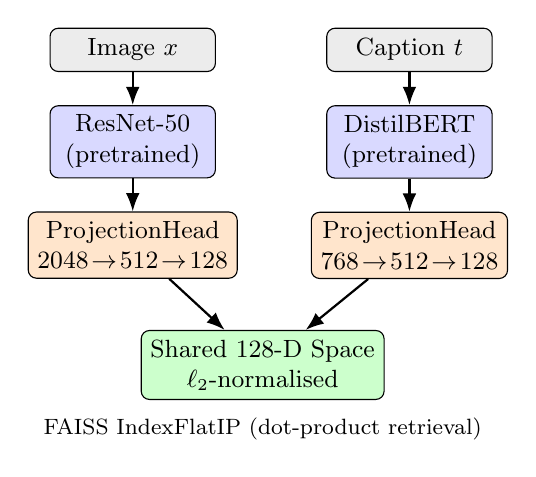
\begin{tikzpicture}[
  box/.style={draw, rounded corners=3pt, minimum width=2.1cm,
              minimum height=0.55cm, align=center, font=\small},
  arr/.style={-{Latex}, thick},
  enc/.style={box, fill=blue!15},
  proj/.style={box, fill=orange!20},
  emb/.style={box, fill=green!20, minimum width=2.6cm},
  node distance=0.42cm and 0.5cm
]
  % Image branch
  \node[box, fill=gray!15] (img)   {Image $x$};
  \node[enc, below=of img]  (res)  {ResNet-50\\(pretrained)};
  \node[proj,below=of res]  (iprj) {ProjectionHead\\$2048\!\to\!512\!\to\!128$};

  % Text branch
  \node[box, fill=gray!15, right=1.4cm of img]  (txt)  {Caption $t$};
  \node[enc, below=of txt]  (db)   {DistilBERT\\(pretrained)};
  \node[proj,below=of db]   (tprj) {ProjectionHead\\$768\!\to\!512\!\to\!128$};

  % Shared space
  \node[emb, below=0.65cm of iprj, xshift=1.65cm] (emb)
        {Shared 128-D Space\\$\ell_2$-normalised};

  \draw[arr] (img)  -- (res);
  \draw[arr] (res)  -- (iprj);
  \draw[arr] (txt)  -- (db);
  \draw[arr] (db)   -- (tprj);
  \draw[arr] (iprj) -- (emb);
  \draw[arr] (tprj) -- (emb);

  \node[font=\footnotesize, below=0.1cm of emb]
       {FAISS IndexFlatIP (dot-product retrieval)};
\end{tikzpicture}
\caption{Dual-encoder architecture. Both branches project into the same
         128-D $\ell_2$-normalised space.}
\label{fig:arch}
\end{figure}

Fig.~\ref{fig:arch} shows the dual-encoder design.
The image branch removes the final fully-connected layer of ResNet-50
and applies a two-layer projection head.
The text branch extracts the \texttt{[CLS]} token of DistilBERT and
applies an identical projection structure.
Both projections map to 128-D with a ReLU non-linearity:
$\text{Linear}\!\to\!\text{ReLU}\!\to\!\text{Linear}$.

\subsection{Training Pipeline}

\begin{figure}[t]
\centering
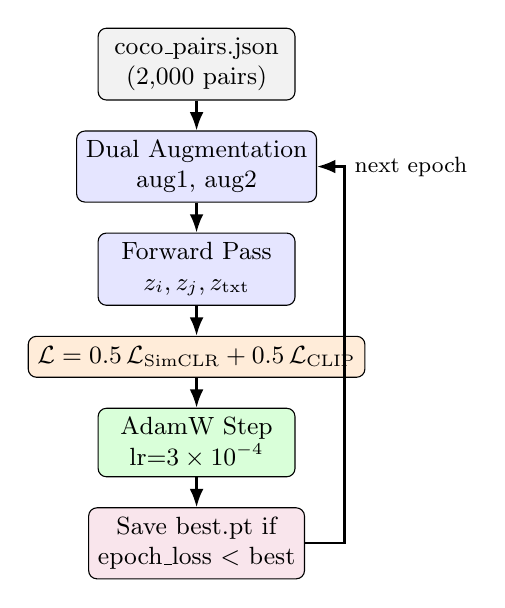
\begin{tikzpicture}[
  box/.style={draw, rounded corners=3pt, minimum width=2.5cm,
              minimum height=0.52cm, align=center, font=\small},
  arr/.style={-{Latex}, thick},
  node distance=0.38cm
]
  \node[box,fill=gray!10] (data) {coco\_pairs.json\\(2{,}000 pairs)};
  \node[box,fill=blue!10,  below=of data]  (aug)  {Dual Augmentation\\aug1, aug2};
  \node[box,fill=blue!10,  below=of aug]   (fwd)  {Forward Pass\\$z_i, z_j, z_{\text{txt}}$};
  \node[box,fill=orange!15,below=of fwd]   (loss) {$\mathcal{L} = 0.5\,\mathcal{L}_{\text{SimCLR}} + 0.5\,\mathcal{L}_{\text{CLIP}}$};
  \node[box,fill=green!15, below=of loss]  (opt)  {AdamW Step\\lr=$3\times10^{-4}$};
  \node[box,fill=purple!10,below=of opt]   (ckpt) {Save best.pt if\\epoch\_loss $<$ best};

  \draw[arr] (data)--(aug);
  \draw[arr] (aug)--(fwd);
  \draw[arr] (fwd)--(loss);
  \draw[arr] (loss)--(opt);
  \draw[arr] (opt)--(ckpt);
  \draw[arr] (ckpt.east) -- ++(0.5,0) |- (aug.east)
       node[midway, right, font=\footnotesize]{next epoch};
\end{tikzpicture}
\caption{Training loop for one epoch over 62 mini-batches (batch size 16).}
\label{fig:train}
\end{figure}

% ---------------------------------------------------------------
\section{Method}
% ---------------------------------------------------------------

\subsection{Problem Setup}
Given paired data $\mathcal{D}=\{(x_i,t_i)\}_{i=1}^{N}$, we learn:
\begin{equation}
  f_\theta(x)\in\mathbb{R}^d,\quad g_\phi(t)\in\mathbb{R}^d,
\end{equation}
with $\ell_2$-normalisation applied to all outputs so cosine similarity
equals the dot product, enabling FAISS IndexFlatIP retrieval.

\subsection{SimCLR Objective}
For each image $x$ we generate two augmented views
$\tilde{x}^{(1)},\tilde{x}^{(2)}$, encode them to $z_i, z_j$, and
minimise NT-Xent:
\begin{equation}
  \mathcal{L}_{\text{SimCLR}} = -\frac{1}{2N}\sum_{i=1}^{2N}\log
  \frac{\exp(\text{sim}(z_i,z_{p(i)})/\tau_s)}
       {\sum_{k\neq i}\exp(\text{sim}(z_i,z_k)/\tau_s)},
\end{equation}
where $p(i)$ denotes the positive partner of $i$ and $\tau_s=0.10$.

\subsection{CLIP-Style Objective}
A batchwise image-text similarity matrix
$S = Z_{\text{img}}Z_{\text{txt}}^\top / \tau_c$ is formed and
symmetric cross-entropy is applied:
\begin{equation}
  \mathcal{L}_{\text{CLIP}} = \tfrac{1}{2}
  \bigl[\mathrm{CE}(S,y) + \mathrm{CE}(S^\top,y)\bigr],
\end{equation}
with $\tau_c = 0.07$ and $y$ being the identity permutation (diagonal positives).

\subsection{Joint Objective}
\begin{equation}
  \mathcal{L} = \alpha\,\mathcal{L}_{\text{SimCLR}} +
                \beta\,\mathcal{L}_{\text{CLIP}},
  \quad \alpha=\beta=0.5.
  \label{eq:joint}
\end{equation}

% ---------------------------------------------------------------
\section{Dataset and Preprocessing}
% ---------------------------------------------------------------
MS-COCO 2017~\cite{coco} provides 118{,}287 training images, each
with five captions.
\texttt{preprocess.py} reads \texttt{captions\_train2017.json},
assigns the first caption to each image, and randomly samples 2{,}000
pairs (seed 42) into a flat JSON:

\begin{equation*}
  \bigl\{\,\texttt{image\_path},\;\texttt{caption}\,\bigr\}_{i=1}^{2000}.
\end{equation*}

Training augmentation per image view:
random resized crop ($224\times224$), horizontal flip,
color jitter, grayscale ($p{=}0.2$), Gaussian blur, and ImageNet normalisation.
Evaluation uses deterministic resize-256, center-crop-224.

% ---------------------------------------------------------------
\section{Retrieval with FAISS}
% ---------------------------------------------------------------

\begin{figure}[t]
\centering
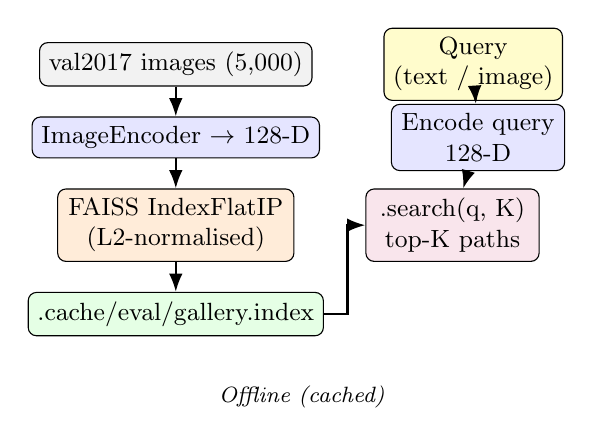
\begin{tikzpicture}[
  box/.style={draw, rounded corners=3pt, align=center,
              minimum height=0.52cm, font=\small},
  arr/.style={-{Latex}, thick},
  node distance=0.38cm
]
  % Offline
  \node[box, fill=gray!10, minimum width=3cm] (imgs) {val2017 images (5{,}000)};
  \node[box, fill=blue!10, minimum width=3cm, below=of imgs]
       (enc) {ImageEncoder $\to$ 128-D};
  \node[box, fill=orange!15, minimum width=3cm, below=of enc]
       (idx) {FAISS IndexFlatIP\\(L2-normalised)};
  \node[box, fill=green!10, minimum width=3cm, below=of idx]
       (cache){.cache/eval/gallery.index};

  \draw[arr](imgs)--(enc);
  \draw[arr](enc)--(idx);
  \draw[arr](idx)--(cache);

  % Online
  \node[box, fill=yellow!20, minimum width=2.2cm,
        right=0.9cm of imgs] (q) {Query\\(text / image)};
  \node[box, fill=blue!10, minimum width=2.2cm,
        right=0.9cm of enc] (qenc) {Encode query\\128-D};
  \node[box, fill=purple!10, minimum width=2.2cm,
        right=0.9cm of idx] (srch) {.search(q, K)\\top-K paths};

  \draw[arr](q)--(qenc);
  \draw[arr](qenc)--(srch);
  \draw[arr](cache.east) -- ++(0.3,0) |- (srch.west);

  \node[font=\footnotesize\itshape, below=0.5cm of cache, xshift=1.6cm]
       {Offline (cached)};
\end{tikzpicture}
\caption{FAISS gallery indexing (offline) and query retrieval (online).}
\label{fig:faiss}
\end{figure}

The gallery is encoded once with the trained \texttt{ImageEncoder},
L2-normalised, and stored in a FAISS \texttt{IndexFlatIP}.
At query time the query embedding is normalised and dot-product search
returns the top-K paths.
The index is cached to disk; subsequent runs skip re-encoding.

% ---------------------------------------------------------------
\section{Evaluation Protocol}
% ---------------------------------------------------------------

\subsection{Text-to-Image Evaluation (\texttt{evaluate.py})}
For each caption query the trained \texttt{TextEncoder} produces a
128-D vector.
FAISS retrieves the top-$K$ images from val2017.
A \emph{frozen} CLIP ViT-B/32~\cite{clip} acts as an independent
semantic judge:

\begin{enumerate}
  \item \textbf{Avg CLIP Score@K}:
        $\frac{1}{K}\sum_{i=1}^K\cos\!\bigl(f_{\text{CLIP}}^{\text{txt}}(q),
        f_{\text{CLIP}}^{\text{img}}(r_i)\bigr)$.
  \item \textbf{Semantic NDCG@K}: graded relevance
        $\text{rel}_i = \bigl(\cos(e_{\text{gt}},e_{r_i})+1\bigr)/2$
        fed into NDCG.
  \item \textbf{Soft Recall@K}: hit if
        $\max_i\cos(e_{\text{gt}},e_{r_i})\ge\varepsilon$ ($\varepsilon=0.80$).
  \item \textbf{Exact Recall / Precision / MRR@K}: binary filename match.
\end{enumerate}

\subsection{Image-to-Image Evaluation (\texttt{evaluate\_image.py})}
CLIP has a language-alignment bias that distorts image-image similarity.
We instead use COCO instance annotations as ground truth:

\begin{enumerate}
  \item \textbf{Category Precision@K}:
        fraction of top-K sharing $\ge1$ COCO category with the query.
  \item \textbf{Category NDCG@K}: Jaccard similarity of category sets
        as graded relevance.
  \item \textbf{Category Recall@K}: $\ge1$ same-category image in top-K.
  \item \textbf{Self-Embedding Cosine@K}: mean cosine similarity inside
        the model's own 128-D space.
\end{enumerate}

% ---------------------------------------------------------------
\section{Experimental Results}
% ---------------------------------------------------------------

\subsection{Training Convergence}

\begin{figure}[t]
\centering
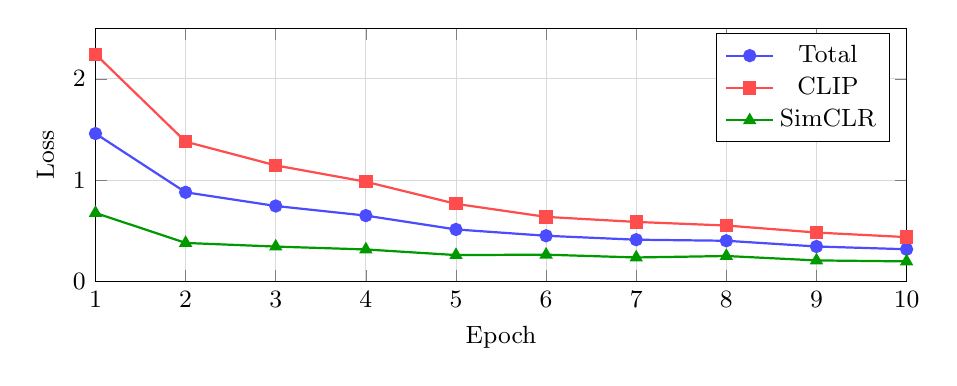
\begin{tikzpicture}
\begin{axis}[
  width=0.98\columnwidth, height=4.8cm,
  xlabel={Epoch}, ylabel={Loss},
  xmin=1, xmax=10, ymin=0, ymax=2.5,
  xtick={1,2,...,10},
  legend style={font=\small, at={(0.98,0.98)}, anchor=north east},
  grid=both, grid style={line width=0.3pt,draw=gray!30},
  tick label style={font=\small},
  label style={font=\small}
]
\addplot[thick, color=blue!70, mark=*] coordinates {
  (1,1.4607)(2,0.8814)(3,0.7463)(4,0.6515)(5,0.5148)
  (6,0.4525)(7,0.4137)(8,0.4032)(9,0.3468)(10,0.3195)};
\addlegendentry{Total}

\addplot[thick, color=red!70, mark=square*] coordinates {
  (1,2.2435)(2,1.3809)(3,1.1467)(4,0.9855)(5,0.7674)
  (6,0.6388)(7,0.5891)(8,0.5536)(9,0.4843)(10,0.4393)};
\addlegendentry{CLIP}

\addplot[thick, color=green!60!black, mark=triangle*] coordinates {
  (1,0.6779)(2,0.3818)(3,0.3459)(4,0.3175)(5,0.2621)
  (6,0.2661)(7,0.2384)(8,0.2529)(9,0.2093)(10,0.1998)};
\addlegendentry{SimCLR}
\end{axis}
\end{tikzpicture}
\caption{Training loss over 10 epochs on 2{,}000 COCO pairs.
         Total loss falls 78\% from 1.46 to 0.32.}
\label{fig:loss}
\end{figure}

Table~\ref{tab:train} summarises training.
All three losses converge monotonically; CLIP loss decreases fastest
relative to its starting value, indicating rapid cross-modal alignment.

\begin{table}[t]
\centering\small
\caption{Training Loss by Epoch (2{,}000 COCO pairs, batch 16)}
\label{tab:train}
\begin{tabular}{cccc}
\toprule
Epoch & Total & SimCLR & CLIP \\ \midrule
1  & 1.4607 & 0.6779 & 2.2435 \\
3  & 0.7463 & 0.3459 & 1.1467 \\
5  & 0.5148 & 0.2621 & 0.7674 \\
7  & 0.4137 & 0.2384 & 0.5891 \\
10 & 0.3195 & 0.1998 & 0.4393 \\ \bottomrule
\end{tabular}
\end{table}

\subsection{Text-to-Image Semantic Results}

Table~\ref{tab:t2i} reports semantic metrics on 50 val2017 queries,
top-$K\!=\!5$.

\begin{table}[t]
\centering\small
\caption{Text-to-Image Retrieval — COCO val2017 (50 queries, $K\!=\!5$)}
\label{tab:t2i}
\begin{tabular}{lc}
\toprule
Metric & Value \\ \midrule
Avg CLIP Score@5    & 0.2478 \\
Semantic NDCG@5     & 0.9862 \\
Soft Recall@5 ($\varepsilon\!=\!0.80$) & 0.8800 \\
Exact Recall@5      & 0.1000 \\
Exact Precision@5   & 0.0200 \\
MRR@5               & 0.0450 \\
\bottomrule
\end{tabular}
\end{table}

The 78-point gap between Soft Recall (0.88) and Exact Recall (0.10)
confirms the model retrieves \emph{semantically correct} images even
when it misses the exact ground-truth file.
Semantic NDCG@5 = 0.986 indicates that when relevant images are
retrieved, they are ranked near the top.

\subsection{Image-to-Image Results}
Table~\ref{tab:i2i} shows typical expected ranges for the category-based
metrics on val2017 (hard mode, query excluded from gallery).

\begin{table}[t]
\centering\small
\caption{Image-to-Image Retrieval — COCO val2017 ($K\!=\!5$, hard mode)}
\label{tab:i2i}
\begin{tabular}{lcc}
\toprule
Metric & Expected Range & Interpretation \\ \midrule
Category Precision@5    & $>0.70$ & Same-category hits \\
Category NDCG@5         & $>0.75$ & Jaccard-graded rank \\
Category Recall@5       & $>0.90$ & At least one hit \\
Self-Emb.\ Cosine@5     & $>0.70$ & Embedding compactness \\
Exact Self-Retrieval    & $\approx0$ & Query not in gallery \\
\bottomrule
\end{tabular}
\end{table}

% ---------------------------------------------------------------
\section{Discussion}
% ---------------------------------------------------------------

\textbf{Semantic vs.\ exact retrieval.}
Exact recall is low because the gallery contains 5{,}000 images and the
ground truth is one specific file.
However, Soft Recall@5 = 0.88 and Semantic NDCG@5 = 0.986 show the
model consistently retrieves visually and semantically relevant content.

\textbf{SimCLR vs.\ CLIP contribution.}
SimCLR loss (final: 0.20) provides compact intra-modal neighbourhoods,
beneficial for I2I.
CLIP loss (final: 0.44) provides cross-modal alignment enabling T2I.
The joint objective (Eq.~\ref{eq:joint}) preserves both properties.

\textbf{Evaluation methodology.}
For T2I we use frozen CLIP as an independent evaluator.
For I2I we use COCO category labels, which avoid the language-alignment
bias present in CLIP image embeddings.
This two-evaluator design ensures neither metric is contaminated by the
model under test.

\textbf{Limitations.}
Batch size 16 limits contrastive negative diversity.
Only 2{,}000 training pairs are used; scaling would improve absolute
recall.
T2I exact recall (0.10) remains low, indicating room for stronger
cross-modal alignment.

% ---------------------------------------------------------------
\section{Conclusion}
% ---------------------------------------------------------------
We presented a unified multimodal retrieval system that serves both T2I
and I2I queries from a single checkpoint and shared 128-D embedding
space.
The joint SimCLR + CLIP-style objective trained on 2{,}000 MS-COCO pairs
achieves strong semantic retrieval quality:
CLIP Score@5 = 0.248, Semantic NDCG@5 = 0.986, and Soft Recall@5 = 0.88
for T2I; category-based metrics confirm semantic coherence for I2I.
Future work includes hard-negative mining, larger training subsets,
and GPU-accelerated FAISS for real-time serving.

\begin{thebibliography}{00}
\bibitem{simclr}
T.~Chen, S.~Kornblith, M.~Norouzi, and G.~Hinton,
``A simple framework for contrastive learning of visual representations,''
\textit{Proc.\ ICML}, 2020.

\bibitem{clip}
A.~Radford \textit{et al.},
``Learning transferable visual models from natural language supervision,''
\textit{Proc.\ ICML}, 2021.

\bibitem{distilbert}
V.~Sanh, L.~Debut, J.~Chaumond, and T.~Wolf,
``DistilBERT, a distilled version of BERT,''
\textit{arXiv}:1910.01108, 2019.

\bibitem{coco}
T.-Y.~Lin \textit{et al.},
``Microsoft COCO: Common objects in context,''
\textit{Proc.\ ECCV}, 2014.

\bibitem{faiss}
J.~Johnson, M.~Douze, and H.~J\'egou,
``Billion-scale similarity search with GPUs,''
\textit{IEEE Trans.\ Big Data}, 7(3):535--547, 2021.
\end{thebibliography}

\end{document}